\section{Zapoznanie z~alokatorem stron}

Ponieważ mechanizm CMA w~dużym stopniu integruje się z~podsystemem
zarządzania pamięci, do jego zrozumienia potrzeba ogólnej wiedzy na
temat tego w~jaki sposób jądro śledzi i~przydziela pamięć procesom
i~sterownikom.

Linux posiada wiele mechanizmów alokacji pamięci.  Począwszy od
najprostszych w~użyciu funkcji \code|kmalloc| i \code|vmalloc|,
poprzez mechanizmy puli pamięci, aż do alokatora czasu bootowania
i~alokatorów pamięci dostępnej dla urządzeń zewnętrznych
\autocite[rozdział 8]{bib:ldd3}.  Pomimo tak dużej liczby interfejsów,
wiele z~nich sprowadza się do wywołania alokatora stron, który jest
sercem podsystemu zarządzania pamięcią.

\subsection{Algorytm bliźniaków}

Alokator stron implementuje algorytm bliźniaków (skąd też jego inna
angielska nazwa: {\it buddy system} lub {\it buddy allocator}), który
operuje na blokach o~rozmiarze $2^k$ jednostek.  W~przypadku Linuksa
jednostką jest pojedyncza strona fizyczna, a~na $k$~narzucone jest
ograniczenie $k < \mathrm{MAX\_ORDER}$.  \code|MAX_ORDER| zależy od
architektury, na którą Linux jest kompilowany, ale zazwyczaj ma
wartość $11$ (toteż na potrzeby tej pracy zakładam, iż $0 \le k \le
10$).

W~Linuksie, przez $k$ rozumie się rząd strony.  Strona rzędu 0 to
pojedyncza strona fizyczna, strona rzędu 1 to dwie strony fizyczne
itd.\ aż do strony rzędu 10, czy też strony maksymalnego rzędu, która
składa się z~1024 stron fizycznych.  Ogólnie, strona rzędu $n$ składa
się z~dwóch stron rzędu $n-1$.

Funkcja \code|alloc_pages|, która jest interfejsem dla alokatora
stron, przyjmuje jako argument właśnie rząd żądanej strony.  Wynikają
stąd, iż alokator stron nie pozwala alokować obszarów:

\begin{itemize}
\item mniejszy niż jedna strona (4096 bajty),
\item których rozmiar nie jest potęgą dwójki, oraz
\item większych niż \unit[4]{MiB}, przez co nie nadaje się do
  alokowania buforu dla pięciomegapikselowej kamery, czy nawet
  pojedynczej ramki {\it full HD}.
\end{itemize}

\begin{wrapfigure}{o}[1.5cm]{0.3\textwidth}
\begin{center}
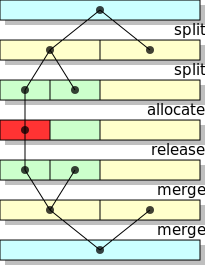
\includegraphics[width=0.25\textwidth]{build/alloc-free-cycle.eps}
\end{center}
\caption[Zarządzanie pamięcią w~algorytmie bliźniaków]{Graficzna
  reprezentacja cyklu alokacji i~zwalniania buforów w~algorytmie
  bliźniaków.}
\end{wrapfigure}

Jak zatem działa algorytm bliźniaków?  Alokator posiada listę wolnych
stron, których rząd jest pomiędzy $0$ a~$10$.  W~Linuksie zrealizowane
jest to poprzez 11 list dwukierunkowych, gdzie każda przeznaczona jest
dla stron o~konkretnym rzędzie.

Gdy sterownik chce zaalokować stronę rzędu $n$, alokator sprawdza
odpowiednią listę.  Jeżeli jest ona pusta, przechodzi do listy ze
stronami rzędu $n+1$, aż znajdzie wolną stronę (lub dojdzie do
maksymalnego rzędu, co sygnalizuje nieudaną alokację).  Jeżeli
uzyskana w~ten sposób strona ma rząd większy niż żądany, jest ona
dzielona na pół, aż do osiągnięcia żądanego rozmiaru.  Strony, które
powstały na skutek podziału większej strony na pół, nazywamy stronami
bliźniaczymi.  Cały proces ilustruje algorytm \ref{alg:buddy-alloc}.

\begin{algorithm}[p]
\caption[Alokacja strony w~algorytmie bliźniaków.]{Alokacja strony
  rzędu $k$ w~algorytmie bliźniaków.}
\label{alg:buddy-alloc}
\begin{algorithmic}[1]
\Require $0 \leq k < \mathrm{MAX\_ORDER}$
\Function{AllocatePage}{$k$}
    \State $i \gets k$
    \While {lista stron rzędu $i = \emptyset$}
        \State $i \gets i + 1$
        \If {$i = \mathrm{MAX\_ORDER}$}
            \State \Return $\emptyset$
        \EndIf
    \EndWhile

    \State $p \gets$ strona z listy stron rzędu $i$
    \While {$i \neq k$}
        \State $i \gets i - 1$
        \State podziel $p$ na pół na $p_1$ i $p_2$
        \Comment{Strony $p_1$ i $p_2$ nazywamy stronami bliźniaczymi}
        \State $p \gets p_1$
        \State dodaj $p_2$ do listy stron rzędu $i$
    \EndWhile
    \State \Return $p$
\EndFunction
\end{algorithmic}
\end{algorithm}

Przy zwalnianiu, dopóki to możliwe, strona jest łączona ze swoją
bliźniaczą stroną, dzięki czemu strony są dodawane do listy wolnych
stron o~dużym rzędzie.  Proces ten ilustruje algorytm
\ref{alg:buddy-free}.

\begin{algorithm}[p]
\caption[Zwalnianie strony w~algorytmie bliźniaków.]{Zwalnianie strony
  $p$ rzędu $k$ w algorytmie bliźniaków.}
\label{alg:buddy-free}
\begin{algorithmic}[1]
\Procedure{FreePage}{$p$, $k$}
    \While {$k + 1 \neq \mathrm{MAX\_ORDER} \wedge p$ posiada wolną stronę bliźniaczą}
        \State $p' \gets$ strona bliźniacza $p$
        \State usuń $p'$ z~listy wolnych stron
        \State $k \gets k + 1$
        \State $p~\gets$ strona powstała w~wyniku połączenia $p$ i~$p'$ \label{alg:buddy-free:join}
    \EndWhile
    \State dodaj $p$ do listy wolnych stron rzędu $k$ \label{alg:buddy-free:add}
\EndProcedure
\end{algorithmic}
\end{algorithm}

\begin{algorithm}
\caption[Alokacja z~uwzględnieniem typu migracji.]{Alokacja strony
  rzędu $k$ z~uwzględnieniem typu migracji $m$}
\label{alg:buddy-fallback}
\begin{algorithmic}[1]
\Function{ChangeBlockMigrateType}{$b$, $m$}
\State zmień typ migracji $b$ na $m$
\ForAll {wolnych stron $p \in b$}
    \State przenieś $p$ na listę wolnych stron typu $m$
\EndFor
\EndFunction
\Statex
\Function{AllocPageMigrateType}{$k$, $m$}
    \State $f \gets$ lista zapasowych typów migracji dla typu $m$
    \State dodaj $m$ na początek $f$
    \ForAll{$m' \in f$}
        \State $p \gets$ \Call{AllocPage}{$k$} biorąc pod uwagę listy stron typu $m'$
        \If {$p \neq \emptyset$}
            \If {$m \neq m' \wedge k \geq \nicefrac{\mathrm{page\_order}}{2}$}
                \State $b \gets$ blok stron zawierający $p$
                \State \Call{ChangeBlockMigrateType}{$b$, $m$}
            \EndIf
            \State \Return $p$
        \EndIf
    \EndFor
    \State \Return $\emptyset$
\EndFunction
\end{algorithmic}
\end{algorithm}
Dokładniejszy opis algorytmu bliźniaków oraz przedstawienie jego
właściwości można znaleźć na stronach 435--455
\autocite{bib:taocp-fa}, a~jego zastosowanie w~Linuksie w~podrozdziale
8.1.7 \autocite{bib:utlk}.


\subsection{Migracja, typy migracji i~bloki stron}\label{sec:migratetype}

Istotnym elementem alokatora stron pominiętym z~opisu w~poprzednim
podrozdziale są typy migracji, których jest sześć: {\it unmovable},
{\it reclaimable}, {\it movable}, {\it cma}, {\it reserve} oraz {\it
  isolate}.

\begin{itemize}
\item Dla potrzeb tej pracy typy {\it unmovable}, {\it
  reclaimable} i~{\it reserve} jak jeden typ -- typ nieruchomy.  To
  uproszczenie wynika z~faktu, iż dla mechanizmu CMA istotne jest
  tylko rozróżnienie pomiędzy stronami ruchomymi i~nieruchomymi.
\item Strony które są typu ruchomego charakteryzują się tym, że ich
  adres fizyczny nie jest istotny, w~związku z~czym mogą być
  przeniesione w~inne miejsce pamięci RAM.
\item Typ {\it cma} jest nowym typem dodanym dla potrzeb interfejsu
  CMA i~jest opisany dokładniej w~podrozdziale \ref{sec:migrate-cma}.
\item Typ {\it isolate} jest niejako pseudo-typem, gdyż jeżeli wolna
  strona ma taki typ, nie może ona zostać zaalokowana.  Więcej na
  temat sposobu w~jaki ten typ może być wykorzystywany opisuję
  w~podrozdziale \ref{sec:alloc-contig-range}.
\end{itemize}

Jednym z~przykładów stron ruchomych są strony anonimowe działających
procesów.  Ponieważ program odwołują się do nich poprzez mapowania
wirtualne, o~ile tablice translacji zostaną uaktualnione, zawartość
strony może być przeniesiona w~dowolne inne miejsce.  Podobnie wygląda
sprawa z~buforami dyskowymi i~wieloma innymi strukturami, którymi
zarządza jądro.

Proces przenoszenia ruchomej strony nazywa się migracją
i wykorzystywany jest między innymi przy obsłudze hot-swapu pamięci,
a~także w~trackie procesu zagęszczania \autocite{bib:compaction,
  bib:supporting-large-contig-regions}, którego celem jest zwiększenie
liczby dostępnych stron o~wysokich rzędach.

Najbardziej skomplikowanym krokiem migracji jest uaktualnienie odwołań
do strony tak, aby wskazywały na nową stronę.  Ponieważ istnieje wiele
rodzajów stron ruchomych (strony anonimowe, bufory dyskowe itp.), jest
to krok specyficzny dla danej strony.

Wołając funkcję \code|alloc_pages|, typ migracji strony jest
przekazywany jako argument, co pozwala alokatorowi stron grupować
strony tego samego typu.  Jest to istotne, gdyż mechanizm zagęszczania
nie działa zbyt dobrze jeżeli ruchome strony przeplatają się
z~pozostałymi stronami, które nie podlegają migracji.

Grupowanie realizowane jest poprzez podział pamięci na bloki
składające się z~1024 stron (choć liczba ta zależy od architektury
i~opcji konfiguracyjnych jądra), jak to pokazuje rysunku
\ref{fig:pages}.  Każdy blok stron ma przypisany typ migracji,
a~alokator stron posiada oddzielne listy wolnych stron dla każdego
typu migracji.  Analizując algorytm \ref{alg:buddy-alloc} należy zatem
brać pod uwagę, iż rozpatruje on listy wolnych stron danego typu
migracji.

\begin{figure}[btp]
\begin{center}
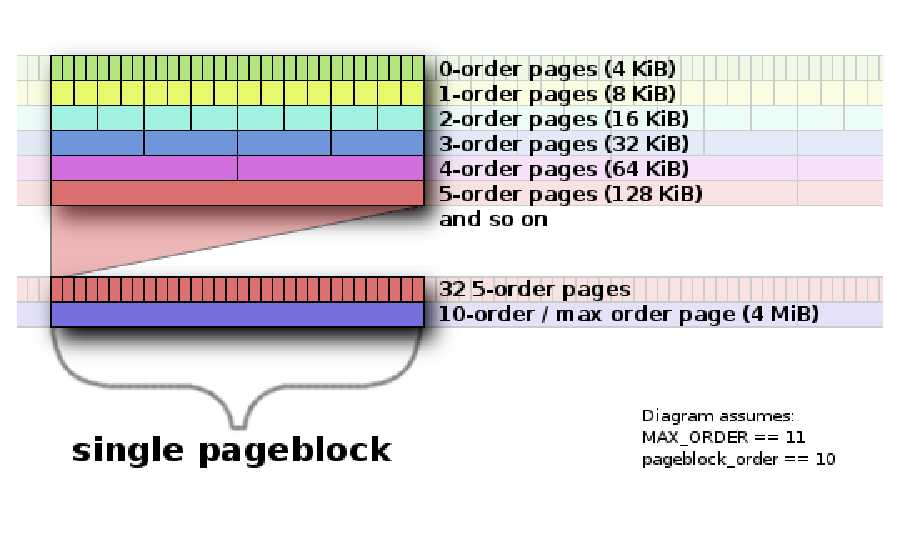
\includegraphics[width=\textwidth]{build/pages.eps}
\end{center}
\caption[Organizacja pamięci w~Linuksie.]{Graficzna reprezentacja
  organizacji stron pamięci stosowanej w~podsystemie zarządzania
  pamięcią Linuksa.}
\label{fig:pages}
\end{figure}


\subsection{Zmiana typu migracji}\label{sec:type-change}

Należy pamiętać, iż dla jądra zrealizowanie alokacji jest ważniejsze
od trzymania stron o~tym samym typie migracji razem.  Dlatego dla
każdego typu migracji istnieje lista zapasowych typów migracji.
Jeżeli alokacja dla żądanego typu migracji nie powiedzie się, alokator
stron będzie próbował z~kolejnymi typami z~list, tak jak to pokazuje
algorytm \ref{alg:buddy-fallback}.

Co więcej, jeżeli rząd żądanej strony jest dostatecznie duży, typ
migracji wszystkich wolnych stron w~danym bloku zostaje zmieniano na
ten zgodny z~wywołaniem funkcji \code|alloc_pages|.

Podczas zwalniania, gdy strona jest dodawana do listy wolnych stron
(widoczne w~linii \ref{alg:buddy-free:add} algorytmu
\ref{alg:buddy-free}) typ migracji listy, na którą strona trafia
determinowany jest poprzez typ migracji przypisany blokowi stron do
którego dana strona należy.

Istotne jest tutaj, aby zauważyć, iż bloki stron mogą zmieniać swój
typ migracji, a~także, że nawet jeżeli blok ma dany typ migracji,
strony o~innym typie migracji mogą być z~niego przydzielone.
